\documentclass{llncs}
%
\usepackage{makeidx}  % allows for indexgeneration
\usepackage{graphicx}        % standard LaTeX graphics tool
                             % when including figure files

\usepackage{multicol}        % used for the two-column index
\usepackage[bottom]{footmisc}% places footnotes at page bottom
\usepackage{amsmath,epsfig}
\usepackage{algorithm}
\usepackage{algorithmic}
\usepackage{subfigure}
\usepackage{multirow}
\usepackage{url}


\begin{document}
\title{ Unreliable Heterogeneous Workers in EvoSpace }
%
\titlerunning{Unreliable Heterogeneous Workers in EvoSpace}  % abbreviated title (for running head)
%                                     also used for the TOC unless
%                                     \toctitle is used
%
\author{--}

\maketitle              % typeset the title of the contribution

\begin{abstract}
TO DO
\keywords{Distributed Evolutionary Algorithms, Cloud Computing}
\end{abstract}
%
\section{Introduction}
\label{sec:intro}
Information technology has become ubiquitous in today's world, sources of computing power range from personal computers and smart-devices to massive data centers. Users can now access vast computational resources available on the Internet using diverse technologies, including cloud computing, peer-to-peer (P2P), and http-based environments. This trend can favor Evolutionary Computation (EC) algorithms as these can be designed as parallel, distributed, and asynchronous systems.
Several Evolutionary Algorithms (EA) have been proposed that distribute the evolutionary process among heterogeneous devices, not only among controlled  nodes in a in-house cluster or grid but also those out side the data center in  users' web browsers and smart phones or external cloud based virtual machines. This reach out approach allows researchers the use of low cost computational power that would not be available otherwise, but on the other hand, have the challenge to manage heterogeneous unreliable computing resources. Lost connections, low bandwidth communications, abandoned work, security and privacy issues are all common? in these settings. 

In this paper the effect of node unavailability in algorithms using the EvoSpace population storage is assessed. EvoSpace \cite{Evospace,FreeLunch}is a framework (that aims?) to implement evolutionary algorithms (EA) using heterogeneous and unreliable resources. EvoSpace is based on Linda's tuple space \cite{Evospace}, a coordination model where each node asynchronously pulls its work from a central shared memory. The core element of EvoSpace is a central repository for the evolving population, that has no knowledge about the evolutionary process. Remote clients, which are here called EvoWorkers, pull random samples of the population to perform on them the basic evolutionary processes (selection, variation and survival), once the work is done, the modified sample is pushed back to the central population. This model contrasts with  the use of a global queue of tasks and implementations of map-reduce algorithms, recently favored in other proposals. Following the tuple space model, when individuals are pulled from the EvoSpace container these are removed from it, so no other EvoWorker could work on them. This design decision has several known benefits relevant to concurrency control in distributed systems, and also is an effective way of distributing the workload. Leaving a copy of the individual in the population server free to be pulled by other EvoWorkers will result in redundant work and this could be costly if the task at hand is time consuming. EvoWorkers are expected to be unreliable, as they can loose a connection or are simply shut down or removed from the client. When an EvoWorker is lost, so are the individuals pulled from the repository. Depending on the type of algorithm been executed, the lost of these samples could have high cost. To address the problem of unreliable EvoWorkers, EvoSpace uses a (simple?) re-insertion mechanism that also prevents the starvation of the population pool. Other pool based algorithms normally use a random insertion technique, but we argue this could negatively impact the outcome of the algorithm (??). This work evaluates the (effect?) of the re-insertion model on the total running time and number of evaluations of a genetic algorithm used to solve a benchmark problem from the P-Peaks problem generator. We compare both approaches: (i) the re-insertion previous individuals at the cost of keeping copies of samples, and (ii) inserting  randomly generated individuals, with the sometimes beneficial cost of adding diversity to the population. For this experiments we use the same (configuration settings?) as an earlier work, in order to compare the performance of the algorithm in similar conditions.
EvoSpace was implemented as a web service on the popular Heroku platform and EvoWorkers where simulated using PiCloud, a scientific computing PaaS. 

The remainder of the paper proceeds as follows. Section \ref{sec:work} reviews related work. Afterwards, Section \ref{sec:evo} briefly describes the proposed EvoSpace framework and gives implementation details the re-insertion process.
The experimental work is presented in Section \ref{sec:experiments}.
Finally, a summary and concluding remarks are in Section \ref{sec:conclusions}.

\section{Related Work}
\label{sec:work}
Using available Internet resources for EC has been the focus of recent research in the field. The use of volunteer computing using BOINC open source software is used by Smaoui et al.  \cite{FekiNG09} in this case BOINC uses redundancy to deal with the volatility of nodes and unreliability of their results. In their work, each BOINC work unit consisted of a fitness evaluation task and multiple replicas were produced and sent to different clients, later when outputs were received a validation step ensured all outputs match. In case of a discrepancy or a time-out from a client, a new job replica was created and sent to another client. The main drawback of this approach was that the master-worker algorithm used was synchronous, so the process had to wait for all jobs to continue to the next generation. Web browsers were used by Merelo et al. [] using Javascript to implement the algorithm, this has the advantage of not requiring the installation of additional software. In this work the server receives an Ajax request with the best individual obtained from the local evolution in clients, and then responds with additional parameters and the best individual in the population so far. If a client is disconnected no special measures are taken. Several cloud-based EC solutions are based on a  global queue of tasks and a Map-Reduce implementation which normally handles failures by the re-execution of tasks \cite{fazenda2012,di2013towards,FlexGP}. 

%% Lo que hice arriba es ir comparando la técnica de failover de cada
%% propuesta me faltan las de abajo 

%This pool-based approach can be traced back to the A-Teams system \cite{ateam}, which is not restricted to evolutionary algorithms.
%Another proposal is made by G. Roy et al. \cite{roy:2009}, who developed a multi-threaded system with a shared memory architecture that is
%executed within a distributed environment and achieves substantial performance gains compared to standard approaches. On the other hand, Bollin and Piastra \cite{bollini:1999} emphasize persistence over performance, proposing a system that decouples population storage from the basic evolutionary operations. A similar decoupled model is proposed by Merelo et al. \cite{merelo:2008}, who used a database to store the population that is accessed through a web-server. The most recent work that is comparable with EvoSpace is the SofEA algorithm proposed by Merelo et al. \cite{sofea1,sofea2}. SofEA is an evolutionary algorithm mapped to a central CouchDB object store. It provides an asynchronous and distributed search process, where the four main evolutionary operators are decoupled from the evolving population.
 
\section{EvoSpace}
\label{sec:evo}
EvoSpace consists of two main components (see figure~\ref{fig:evo}): (i) the EvoSpace container that stores the evolving population and (ii) EvoWorkers, which execute the actual evolutionary process, while EvoSpace acts only as a population repository.
In a basic configuration, EvoWorkers pull a small random subset of the population, and use it as the initial population for a local EA executed on the client machine. Afterwards, the evolved population from each EvoWorker is returned to the EvoSpace container. When individuals are pulled from the container they remain in a phantom state, they cannot be pulled again but they are not deleted. Only if and when the EvoWorker returns the replacement sample phantoms are truly deleted. If the EvoSpace container is at risk of starvation or optionally when a time-out occurs new phantom individuals are re-inserted to the population and available again. This can be done because a copy of each sample is stored in a priority queue used by EvoSpace to re-insert the sample to the central population; similar to games where characters are respawned after a certain time. In the experiments conducted in this work re-insertion occurs when the population size is below a certain threshold. Figure~\ref{fig:evo} illustrates the main components of EvoSpace.

\begin{figure}[!t]
    \centering
        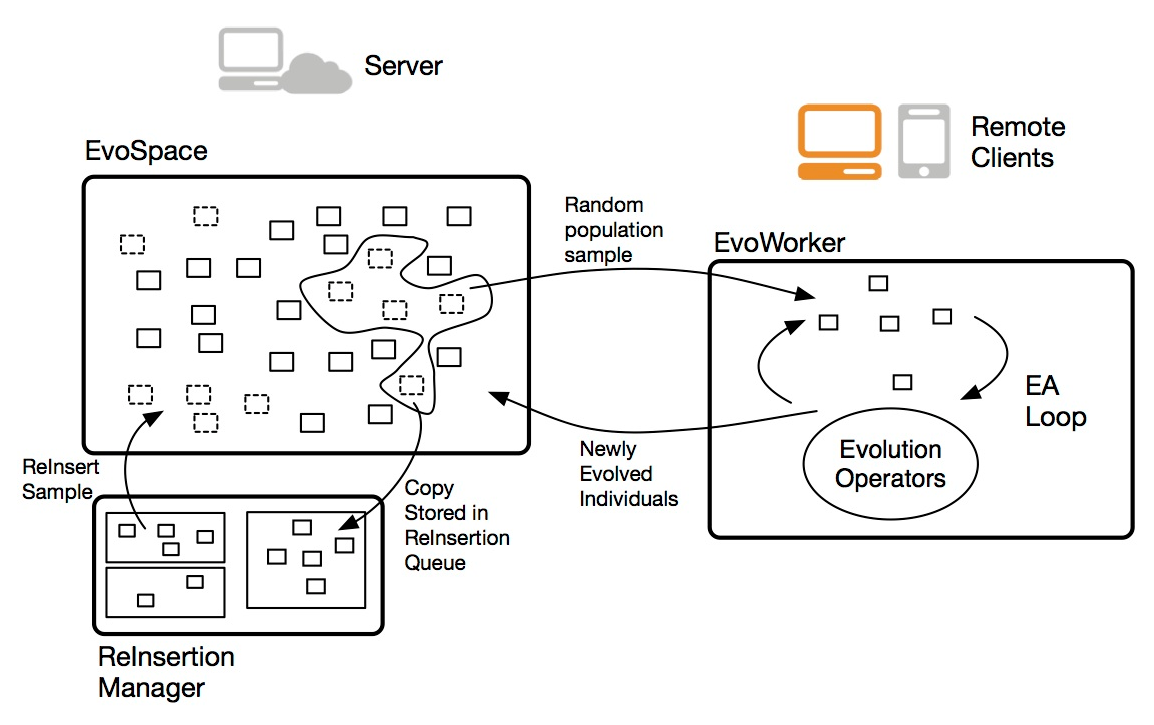
\includegraphics[width=3.5in]{eps/evospaceExample.eps}
    \caption{Main components and dataflow within EvoSpace.}
    \label{fig:evo}
\end{figure}


\subsection{Implementation}
Individuals are stored in-memory, using the Redis key-value database.
Redis was chosen over a SQL-based management system, or other non-SQL alternatives, because it provides a hash based implementation of sets and queues which are natural data structures for the EvoSpace model. The logic of EvoSpace is implemented as a python module exposed as a Web Service using Cherrypy and Django http frameworks. The EvoSpace web service can interact with any language supporting JSON-RPC or Ajax requests. The EvoSpace modules and workers in JavaScript, JQuery and python are available with a Simplified BSD License from https://github.com/evoWeb/EvoSpace. 

\subsection{Evospace as a Heroku Application}
Heroku is a multi-language PaaS, supporting among others
Ruby, Python and Java applications. The basic unit of composition on
Heroku is a lightweight container running a single user-specified
process. These containers, which they call {\em dynos}, can include web
(only these can receive {\tt http} requests) and worker processes
(including systems used for database and queuing, for instance).
These  process types are the prototypes from which one or more dynos can be instantiated;
if the number of requests to the server increases
more instances can be assigned on-the-fly. In our case, our CherryPy web application server
runs in one web process, when the number of workers was increased we added more dynos (instances) of the CherryPy process.
% scaling why? no entiendo lo que significa en este contexto - JJ
% detalle la explicacion
This model is very different from a VPS where users pay for the
whole server; in a process based model, users pay only for the
processes they need.
%deberías usar alguna tipografía para las aplicaciones, \sc
%por ejemplo. O mayúsculas en la primera letra, simplemente - JJ

Once deployed the web process can be scaled up by assigning more dynos; in our case and in the more demanding configurations of our experiments, the web process was scaled to 36 dynos. Instructions and code for deployment is available at \url{http://www.evospace.org/software.html}
% Enlace directo a este código - JJ -resolved
% usa más los puntos y coma, hombre - JJ
% Siii, aunque se supone que los que programamos Python no ocu
\subsection{Evoworkers as PiCloud Jobs}
PiCloud is a PaaS, with deep Python integration; we could work directly from our text editors, and run the application as if it was local. Using a library, Python functions are transparently uploaded to PiCLoud's servers as units of computational work they call \emph{jobs}. Each job is added to a queue, and when there is a core available, the job is assigned to it.Realtime cores can be reserved (for a fee) for certain amount of time, when reserved, cores are available immediately allowing a parallel execution. Both Heroku and PiCloud platforms are deployed  on top of Amazon Web Services (AWS) infrastructure in the US-EAST Region. This ensures minimal latency and a high bandwidth communication between the services, and there is no charge for data transfer costs between both services. The code for the EvoWorkers implementation is publicly available from a github repository \url{http://goo.gl/8Rv5K}.

\section{Experimental work}
\subsection{Benchmark}
\label{ss:benchmark}
The experiment reported here uses a multimodal problem generator to
investigate the performance of the Evospace distributed algorithm in a
cloud based platform. A P-Peaks generator has been chosen because the problem
(and the computing resources needed for the search) can be appropriately scaled.
Proposed by De Jong et al. in \cite{Jong:PS97} a
P-Peaks instance is created by generating a set of P random N-bit
strings, which represent the location of the P peaks in the space. To
evaluate an arbitrary bit string \begin{math} \mathbf{x} \end{math}
first locate the nearest peak (in Hamming space). Then the fitness of
the bit string is the number of bits the string has in common with
that nearest peak, divided by N. The optimum fitness for an individual
is 1. This particular problem generator is a generalization of the
P-peak problems introduced in \cite{Jong:1990}.             % this
                                % problem has been chosen because (no
                                % me sirve porque me lo dijo JJ - JJ
                                % Oh estaba más abajo, pero aquí lo justifico rapidito.

\begin{equation}
f_{P-PEAKS}(\mathbf{x})=\frac{1}{N} \overset{P}{\max_{i=1}} \{N-hamming(\mathbf{x},Peak_i)   \}
\end{equation}

A large number of peaks induce a time-consuming algorithm,
since evaluating every string is computationally hard; this is
convenient since to evaluate these type of distributed evolutionary
algorithms fitness computation has to be significant with respect to
network latency (otherwise, it would always be faster to have a
single-processor version). However
according to Kennedy and Spears \cite{Kennedy:1998ch} the length of
the string being optimized has a greater effect in determining how
easy or hard is the problem. In their experiments an instance having P
= 200 peaks and N = 100 bits per string is considered to produce a
considerably difficult problem. Alba et al. \cite{Alba:2002dq}
considered an instance with greater difficulty with P = 512 peaks and
N = 512, as a benchmark for an heterogenous execution of parallel
genetic algorithms. As our  experiments were going to be executed
using external pay\textendash per\textendash use resources, a moderate
demand problem was configured. Our instance uses P = 256 peaks and N =
512 bits, this configuration requires considerable computational time,
but also within our allocated budgets and considering 30 executions for each of the experiments.

\subsection{Experimental Set-up}
As EvoSpace is only the population store, EvoWorkers must implement the genetic operators. As stated earlier, our objective is to let researchers use the same tools as in their local setting. As a test, the genetic algorithm executed by EvoWorkers has been implemented using the DEAP (Distributed Evolutionary Algorithms in Python) framework \cite{DEAP_JMLR2012}. Only the basic non-distributed GA library was used. Three methods were added to the local algorithm: getSample() and  putBack(); and  another for the  initialization of the population. They simply use DEAP´s methods; for instance to generate the initial population, a local initialize() is called and the population sent to EvoSpace.

The selection of parameters was based on those used in \cite{Alba:2002dq}: a
tournament size of 4 individuals, a crossover rate of 0.85 and a
population of 512 individuals. In  \cite{Jong:PS97} a mutation rate
equal to the reciprocal of the chromosome length; is recommended, as
DEAP uses two parameters they were defined as follows, mutation
probability of 0.5 and an independent flip probability of 0.02. For
EvoWorkers the parameters were 128 worker generations for each
sample, and a sample size of 16. A summary of the setup is presented in table~\ref{params}.

\begin{table}[!t]
\renewcommand{\arraystretch}{1.3}
\caption{GA and EvoWorker parameters for experiments.}
\label{params}
\centering
\begin{tabular}{|l|c|}
\hline
\multicolumn{2}{|c|}{GA Parameters} \\
\hline
Tournament size & 4 \\
Crossover rate & 0.85  \\
Population Size & 512 \\
Mutation probability & 0.5 \\
Independent bit flip probability  & 0.02 \\
\hline
\multicolumn{2}{|c|}{EvoWorker Parameters} \\
\hline
Sample Size & 16 \\
Generations & 128 \\
\hline
\multicolumn{2}{|c|}{Variable Parameters} \\
\hline
PiCloud Worker Type & Realtime, Standard \\
Number of Workers & 2,4,8,16,28 \\
Number of Executions & 30 \\
\hline

\end{tabular}
\end{table}





%
% ---- Bibliography ----
\bibliographystyle{abbrv}
\begin{footnotesize}
\bibliography{biblio}
\end{footnotesize}

\end{document}
